\section{Vårt Arbeid}

\subsection{Forarbeid}

\subsubsection{Design av absoluttverdikrets}

I forarbeidet skulle det designes en 4-bits absoluttverdikrets.
For å ta absoluttverdien av et binært tall kan man invertere det og addere 1.
En absoluttverdikrets kan dermed bygges opp av inverterkretser og av halvadderkretser.
Vi startet med å designe en inverterkrets, altså en krets som inverterer hvert bit som kommer inn, hvis kretsen er aktivert.

Det blir gjort tydelig av tabell \ref{tabell:1} at en slik krets kan lett implementeres som en XOR-port.

\begin{table}[h]
  \centering
  \begin{tabular}{c c|c}

    In & En & Out\\
    \hline
    0 & 0 & 1\\
    0 & 1 & 0\\
    1 & 0 & 1\\
    1 & 1 & 0\\

  \end{tabular}
  \caption{Sannhetstabell for inverterkrets}
  \label{tabell:1}
\end{table}

% \begin{figure}
%   \centering
%   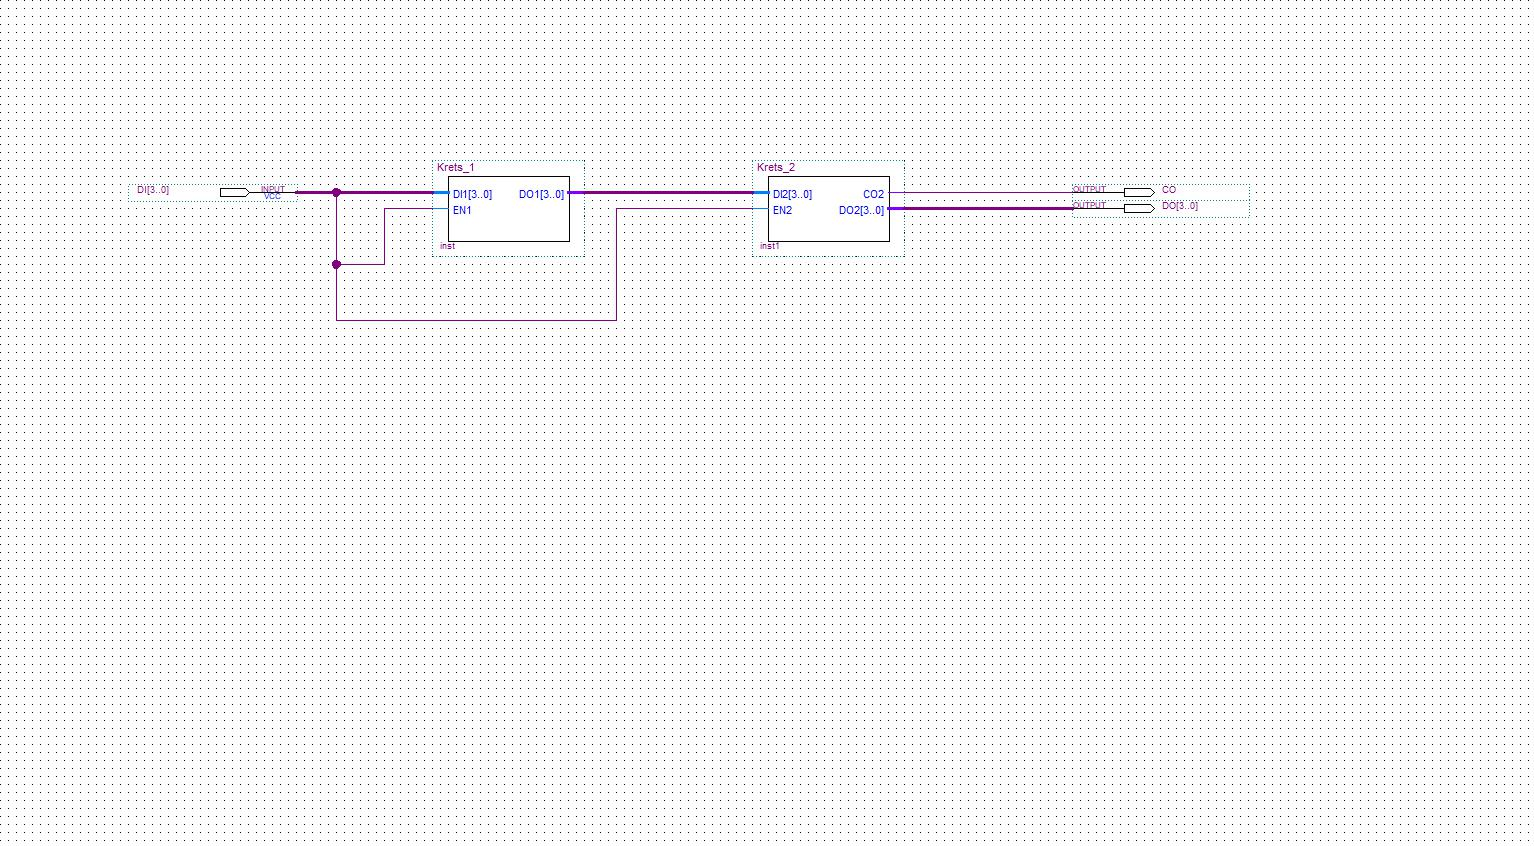
\includegraphics{4 bit abs}
%   \caption{}
%   \label{}
% \end{figure}

Deretter designet vi en halvadderkrets. En halvadderkrets adderer to tall og har to utganger, en for summen og en for mente, så lenge kretsen er aktivert.

\begin{table}[h]
  \centering
  \begin{tabular}{c c|c|c}

    In & Carry-In & Sum & Carry-Out\\
    \hline
    0 & 0 & 0 & 0\\
    0 & 1 & 1 & 0\\
    1 & 0 & 1 & 0\\
    1 & 1 & 0 & 1\\

  \end{tabular}
  \caption{Sannhetstabell for halvadderkrets}
  \label{tabell:2}
\end{table}

% \begin{figure}
%   \centering
%   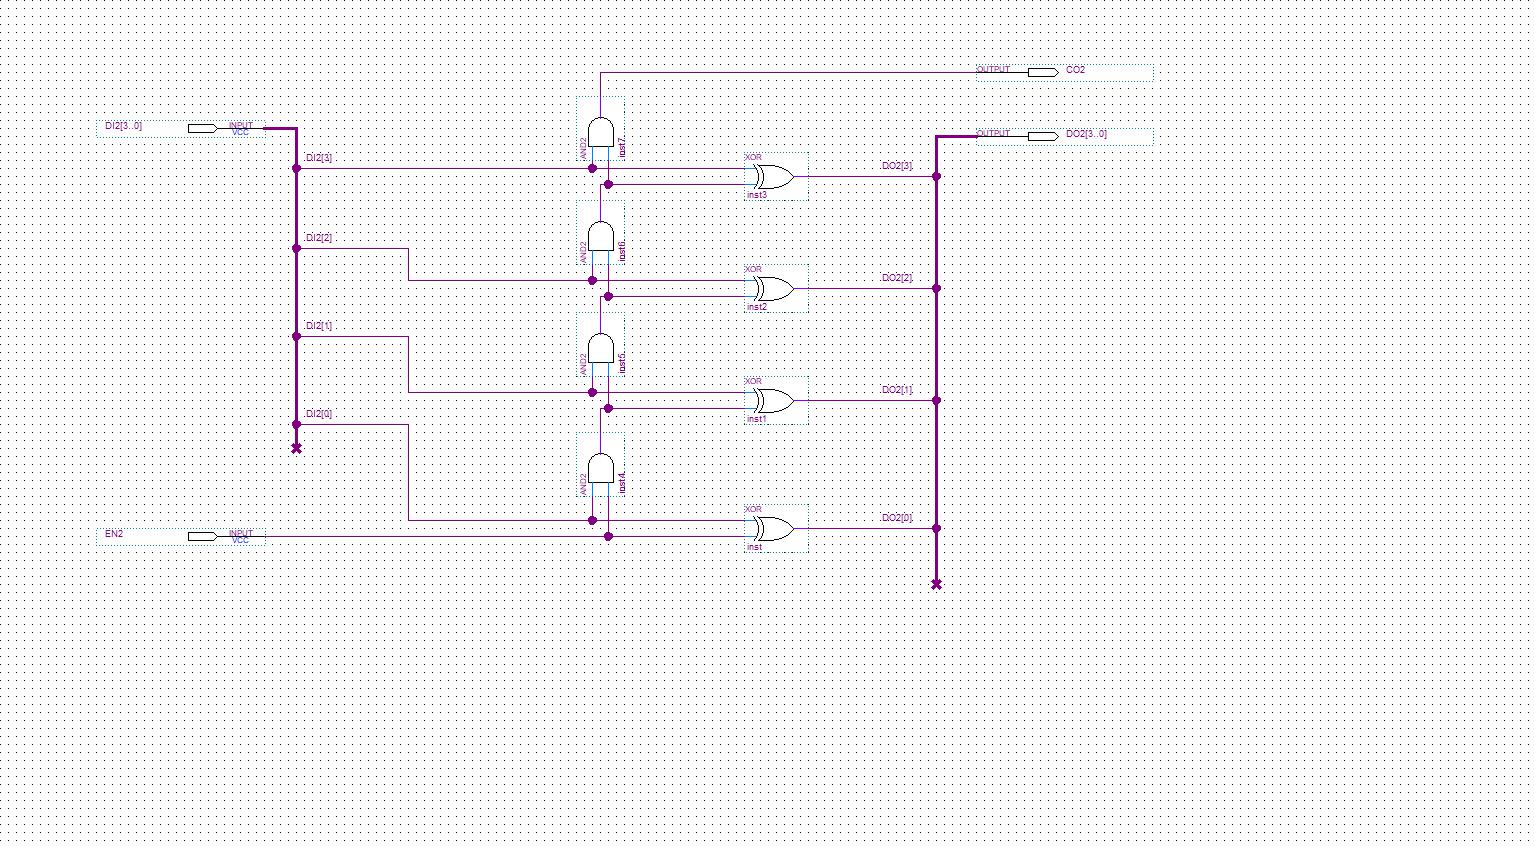
\includegraphics{4 bit adder}
%   \caption{}
%   \label{}
% \end{figure}

Etter å ha designet komponentene til 4-bits absoluttverdikretsen, måtte vi sette disse sammen.
Da lagde vi blokker ved å sette inverterkretsen og halvadderkretsen i serie, og satte fire av disse blokkene i parallell.
Videre brukte vi MSB som enable signal for inverterne og som mente inn for første halvadder, slik som i figur [REF HER]. 

\subsubsection{Jeg må jobbe på toget}
